\documentclass{beamer}
\usepackage{graphicx}
\usepackage{xcolor}
\usepackage{amssymb}
\usepackage{amsfonts}
\usepackage{pifont}
\usepackage{subcaption}
\def\E{\mathbb{E}}
\def\R{\mathbb{R}}
\DeclareMathOperator{\Vol}{Vol}
\newif\ifbeamer
\beamertrue

%further improvement
%background intro added Chen Chuan's work
%simulation add hierarchical method
%find suitable dataset to apply info-clustering
%Yang Li's suggestion: compared with other clustering method, the threshold is the same or not
%early stopping technique, complexity from n -> log(n)
\title{Research Progress Report}
\author{Feng Zhao}
\date{\today}
\begin{document}
\begin{frame}
	\titlepage
\end{frame}


\section{Introduction}

\begin{frame}
\frametitle{Problems}
Compute the probability content $P(H_n)$ of the convex hull $H_n$
of $n$ random points in $\mathbb{R}^d$
\begin{itemize}
\item the random points are i.i.d. sampled from a given distribution $\Gamma$
\item we are more interested in the asymptotic behavior of $P(H_n)$
as $n\to\infty$
\item $P(H_n)$ is different from the expected volume $\mathbb{E}[\Vol]$
\end{itemize}
\end{frame}
\begin{frame}
	\frametitle{Equivalent problem}
    \begin{align}
        P(H_n^c) & = \frac{1}{n+1}\mathbb{E}[V_{n+1}]\\
        F_{n+1} & = V_{n+1} (d-1) - d^2 + d + 2 \textrm{ \textcolor{red}{\ding{55}}}
        \label{eq:FV_d}
    \end{align}   
    \begin{itemize}
    \item We can obtain
    $\mathbb{E}[F_{n+1}]$ and $\mathbb{E}[\Vol]$ for any $d$, 
    \item \eqref{eq:FV_d} comes from Raynaud 1970
    \end{itemize}
\end{frame}   
\begin{frame}
    \frametitle{Special cases}
    $d=1,P(H_n^c) = \frac{2}{n+1}$ for any distribution.
    
    Consider $d$ is fixed, $n\to \infty$.
    \begin{table}
        \begin{tabular}{|c|c|c|c|}
            \hline
            Distribution & $d=2$ & $d=3$ &  general $d$ \\
            \hline
            Uniform sphere & $C_2 n^{-1/3}$ & $C_3 n^{-1/2}$ &
            $C_{d} n^{-2/(d+1)}$ \\
            \hline
            Multivariate Gaussian &
            $2\sqrt{2\pi}\frac{\sqrt{\log n}}{n}$
            & $\frac{4\pi}{\sqrt{3}}\frac{\log n}{n}$
            & 
            \textcolor{purple}{$D_d\frac{(\log n)^{(d-1)/2}}{n}$} \\
            \hline
            Multivariate Cauchy & 
            $\frac{\pi^2}{2}n^{-1}$ &
            $\frac{2\pi^2}{3}n^{-1}$ &
            \textcolor{red}{$E_d n^{-1}$}\\
            \hline
            Multivariate t-distribution &
            $g(v) n^{-1}$ & & \\
            \hline
        \end{tabular}
        \caption{Asymptotic behavior of $P(H_n^c)$}
    \end{table}
    Some known constants:
    \begin{align*}
    g(v) &= \frac{4\sqrt{\pi}
    \Gamma(v+\frac{1}{2})\Gamma^2\left(\frac{v}{2}+1\right)}
    {\Gamma(v+1)\Gamma^2 \left(\frac{v+1}{2} \right)}
    \end{align*}
\end{frame}

\begin{frame}
    \frametitle{Geometric counting in 4d}
    Euler's characteristic (Dehn–Sommerville equations):
    \begin{equation}
        V_N - E_N + F_N - \widetilde{V}_N = 0
    \end{equation}   
    \begin{itemize}
        \item $E_N$: the number of edges
        \item $F_N$: the number of triangular faces
        \item $\widetilde{V}_N$: the number of tetrahedras (tetrahedra)
    \end{itemize}    
    Using $F_N = 2 \widetilde{V}_N$,
    we can obtain $V_N - E_N + F_N = 0$
\end{frame}

\begin{frame}
    \frametitle{The limit of equivalent distribution for convex hull of spherically symmetric samples}
    \begin{itemize}
        \item Eddy and Gale 1981
        \item one to one mapping from a convex hull and functions defined on unit sphere
    \end{itemize}
    \begin{block}{2d example}
        \begin{itemize}
        \item Given random samples $X_1, \dots, X_n$,
        \item The function is defined on $\gamma \in [0,2\pi]$
        $X_i$
        \item Define $b_k(\gamma) =  k_1\cos\gamma + k_2 \sin \gamma$
        \item $D_n(\gamma):=\max_{1\leq i \leq n}\{b_{X_i}(\gamma)\}$
        \end{itemize}
    \end{block}
    Studies the limit distribution of $D_n(\gamma)$ for three types of distributions

    \footnotesize{William~F Eddy and James~D Gale.
     The convex hull of a spherically symmetric sample.
    {\em Advances in Applied Probability}, 13(4):751--763, 1981.
    }
\end{frame}
\begin{frame}
    \frametitle{Three types of spherically symmetric distribution}
    Depending on how $\Pr(R>r)$ decreases as $r\to \infty$
    \begin{itemize}
        \item Algebraic tails: $\Pr(R>r) = r^{-\alpha} L(r)$ where $L(r)$ is a slowly varying function
        \item Exponential tails: $\Pr(R>r) = r^{\alpha} \exp(-\gamma r^{\beta})$, $\gamma$ is scale factor
        \item Truncated tails: $\Pr(R>r) = (1-r)^{\alpha}$ for $r<1$ and $\Pr(R>r)=1$ for $r>1$
    \end{itemize}
\end{frame}
\begin{frame}
    \frametitle{
        2D formula for the expected number of vertices
    }
    \begin{align*}
        \E[V_N]
        & \sim \pi N^2 \int_{\R} F^{N}(x) dx \cdot \int_{\R} |y_1-y_2| f(x, y_1) f(x,y_2)dy_1dy_2
    \end{align*}
    \begin{itemize}
        \item $F(x)$: CDF of the marginal distribution of $X$
        \item $f(x,y)$: joint distribution of $(X,Y)$
    \end{itemize}
    Suppose $\alpha \geq 0$
    \begin{itemize}
        \item Algebraic tails: $p(x,y) = C_{\alpha}(1+x^2+y^2)^{-\alpha-3/2}$,
        $\E[V_N] \sim D_{\alpha}$
        \item Truncated tails: $p(x,y) = C_{\alpha}(1-x^2-y^2)^{\alpha}$ for $r\leq 1$ and $p(x,y)=0$ for $r>1$
        ,$\E[V_N] \sim D_{\alpha} N^{1/(2\alpha + 3)}$ [Affentranger, 1991]
    \end{itemize}
\end{frame}
\begin{frame}{Exponential tails}
    Suppose $\beta > 0$
\begin{equation*}
    p(x,y) = C  \exp(-(x^2+y^2)^{\beta}/2)    
\end{equation*}
Then 
\begin{equation*}
    \E[V_N] \sim D_{\beta} (\log N)^{2-\frac{3}{2\beta}}
\end{equation*}
Idea: approximate the pdf by
$(1+x)^{\alpha} \approx 1+\alpha x$
\begin{equation*}
    \tilde{p}(x,y)=
    C \exp(-x^{2\beta}/2) \exp(-\beta y^2 x^{2\beta-2}/2)
\end{equation*}
\end{frame}
\begin{frame}{Algebraic tails family}
    \begin{itemize}
        \item finite linear combination: the rate depends on the dominant term, e.g.
        \begin{equation*}
            p(x,y) = \sum_{i=1}^k C_i (1+\frac{1}{v_i}(x^2+y^2))^{-v_i/2 - 1}
        \end{equation*}
        \item only the dominant term contributes to the rate, e.g.
        \begin{equation*}
            \E[V_N] \sim g(\min_{1\leq i\leq k} v_i)
        \end{equation*}
        \item Same $\E[V_N]$ with Cauchy distribution
        \begin{equation*}
            p(x,y) = C \log \left(1+\frac{1}{(1+x^2+y^2)^{3/2}} \right)
        \end{equation*}
    \end{itemize}
\end{frame}
\begin{frame}
    \frametitle{Property of $g(v)$}
    \begin{enumerate}
        \item $g(1)=\frac{\pi^2}{2}$
        (2d-Cauchy), $g(0)=4,
        g(v) \sim 2\pi \sqrt{v}$
        as $v\to \infty$
        \item $g(v)$ is monotonic increasing
    \end{enumerate}
    \begin{figure}
        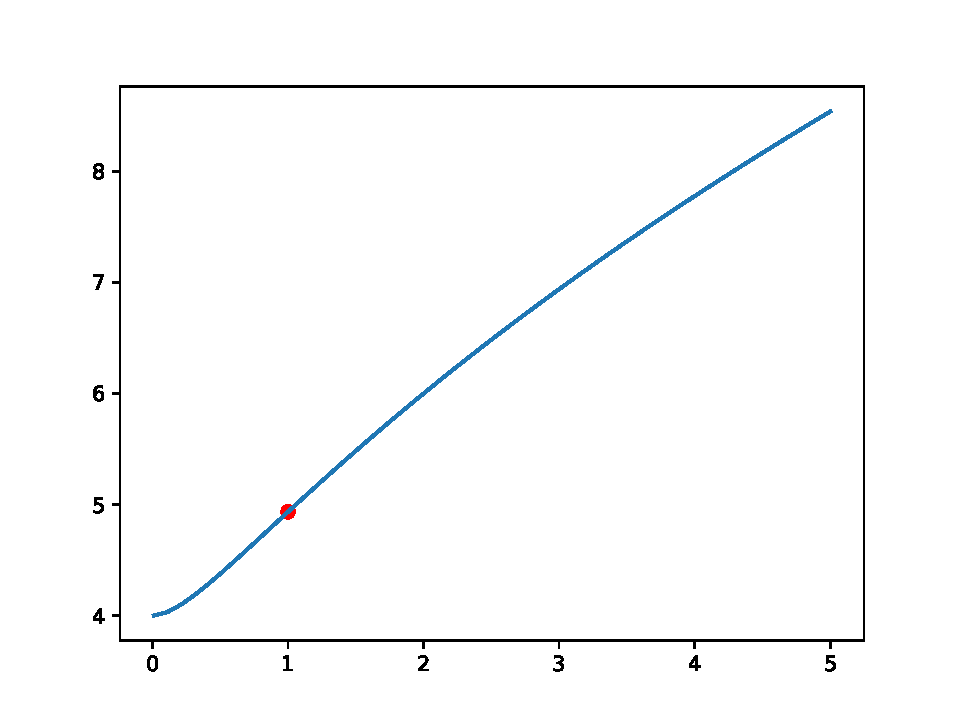
\includegraphics[width=0.6\linewidth]{2d_t_distribution_g_v.pdf}
        \caption{Illustration of $g(v)$. The red point represents the special case for 2d Cauchy.}
    \end{figure}
\end{frame}
\begin{frame}
    \frametitle{Simulation}
    The horizontal red line represents the theoretical coefficient.
    \begin{figure}
        \centering
        \begin{subfigure}[b]{0.5\linewidth}
        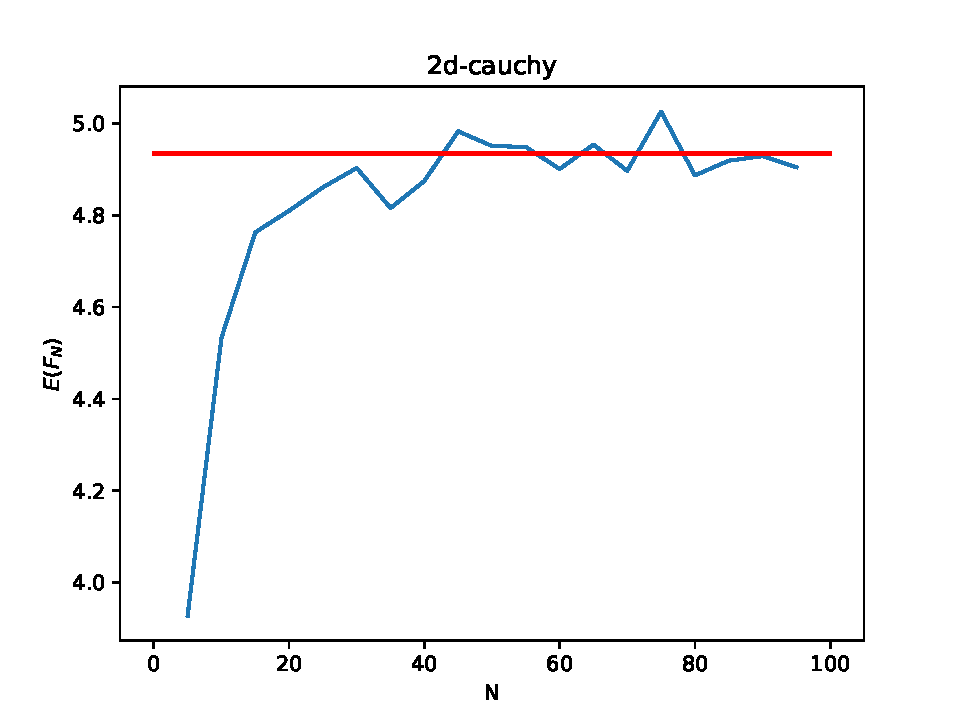
\includegraphics[width=\textwidth]{fig/2d-cauchy.pdf}
        \caption{$d=2$}
        \label{fig:2d_cauchy}
        \end{subfigure}~
        \begin{subfigure}[b]{0.5\linewidth}
          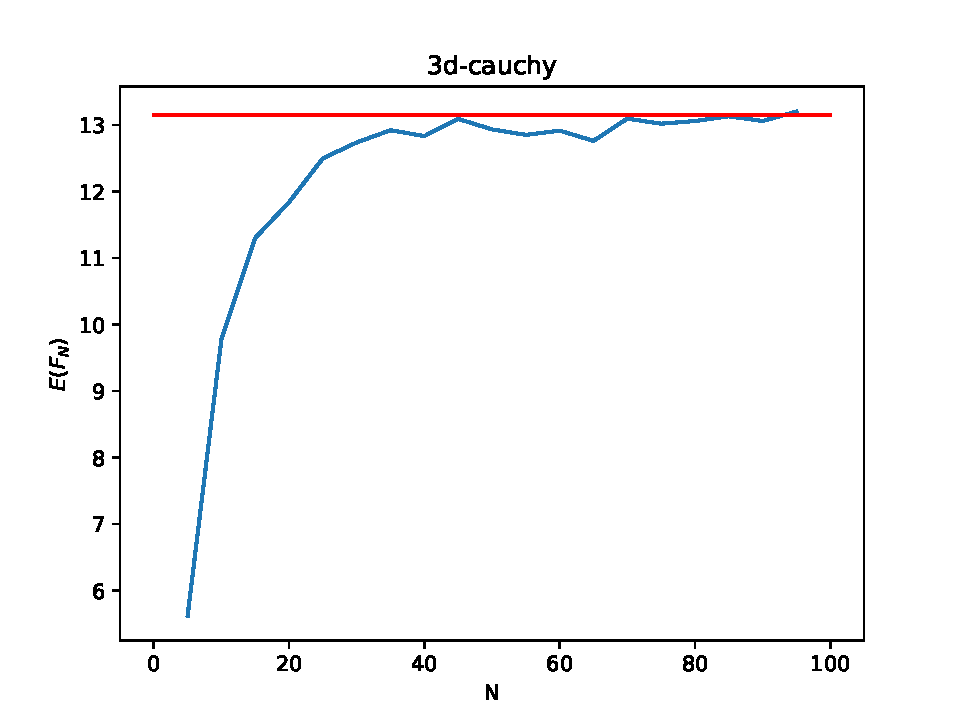
\includegraphics[width=\textwidth]{fig/3d-cauchy.pdf}
          \caption{$d=3$}
          \label{fig:3d_cauchy}
          \end{subfigure}
          \caption{The expected number of faces $E(F_N)$ varies with $n$}
      \end{figure}
\end{frame}
\end{document}
